\section{Профиль и протокол}
\subsection{Цель и теоретические сведения}
Цель работы --- сравнить индуктивные смещения CNN и ViT при сопоставимом числе параметров, изменении объёма train и искажении test. Методика соответствует заданию~\cite{teacher}. Локальное ядро и общие веса CNN задают предположение о пространственной структуре изображения; ViT получает глобальные связи через внимание и обучаемые позиционные вложения.

Для свёртки с ядром $k$, каналами $C,C'$ и выходом $H'\times W'$ число MAC равно $H'W'C'Ck^2$. ViT преобразует патчи $P\times P$ в токены ширины $D$, добавляет CLS и позиционные вложения. Длина последовательности $N'=HW/P^2+1$; в каждом из шести pre-LN блоков применяются внимание и MLP с GELU:
\begin{equation}\operatorname{Attention}(Q,K,V)=\operatorname{softmax}(QK^\top/\sqrt{d_k})V,\quad
C_{block}\approx12N'D^2+2N'^2D.\end{equation}
Здесь $Q,K,V$ --- проекции токенов, $d_k$ --- ширина головы. Квадратичный член объясняет чувствительность стоимости к размеру патча.

Основная метрика --- accuracy; относительное преимущество и падение при искажении заданы как
\begin{equation}\Delta(r)=M_{ViT}(r)-M_{CNN}(r),\quad
\delta_c(s)=\frac{M_{clean}-M_c(s)}{M_{clean}+10^{-12}},\quad
\overline M_c=\frac13\sum_{s=1}^3M_c(s).\end{equation}
Искажение $c$ и уровень $s$ не меняют метки. Для смены лидера обе разности, на чистом test и по $\overline M_c$, должны иметь противоположные знаки и модуль не менее 0.01.

\subsection{Данные и условия обучения}
Использован CIFAR-10, разбиение ЛР0: train 43 000, val 5 000, cal 2 000, test 10 000. Нормализация рассчитана только по train; cal не используется. Вложенные стратифицированные подмножества заданы профилем P3adf02: $r=0.05,0.15,0.30,0.60,1$. Индексы каждого класса один раз перемешаны генератором базового seed. Изменение $r$ только добавляет объекты.

CNN --- ResNet-18 со свёрткой stem $3\times3$, stride 1 и без начального max-pool. ViT имеет $P=4$, $D=384$, шесть блоков и шесть голов, MLP ширины 1536, CLS и обучаемые абсолютные позиции. Предобучение не используется. Общие условия: AdamW, weight decay 0.05, batch 128, ровно $S=10\,000$ обновлений, 5\% прогрева и cosine, FP32 на RTX 3060 Laptop. LR выбрана отдельно по val на полном train из $0.0003,0.001,0.003$: CNN 0.003, ViT 0.0003. Сравнивается архитектура вместе с этим заранее фиксированным рецептом обучения.

Политика A1 --- случайный crop $32\times32$ после padding 4 и горизонтальное отражение. Профиль содержит A2 RandAugment+CutMix, но дополнительные обучающие серии A0/A2 здесь не заявляются. Персональные искажения E2: blur, contrast, patch shuffle.

\section{Ресурсы моделей}
Режим сравнения --- param matched. Число параметров ViT составляет 95.72\% числа параметров CNN, что укладывается в допуск 20\%. Число MAC ViT больше в 1.27965 раза, поэтому равенство вычислений не установлено. Подсчёт включает QKV, выходную проекцию и произведения attention; аналитическая и измеренная суммы совпали.
\begin{table}[H]\centering\footnotesize
\setlength{\tabcolsep}{4pt}
\caption{Ресурсы моделей: FP32, CUDA; время обучения при $r=1$.}\label{tab:resources}
\begin{tabular}{lrrrrrr}
\toprule
Модель & Параметры & MAC, млн & Latency, мс & Объект/с & Train MiB & Train, с \\
\midrule
CNN & 11173962 & 555.42 & 6.399 & 5987.6 & 1993.4 & 1187.95 \\
VIT & 10695562 & 710.75 & 4.644 & 3052.0 & 1912.8 & 1830.35 \\
\bottomrule
\end{tabular}
\end{table}


Latency при $B=1$ и throughput при $B=128$ получены из 30 повторов после 10 прогревов с синхронизацией CUDA. Throughput в этой таблице вычислен по медианному времени собственного batch. Пиковая память относится к обучению. Малый batch CNN показал повышенный разброс времени, поэтому его медиана характеризует данную серию, а не универсальную задержку. При полном train ViT обучался в 1.54076 раза дольше CNN.
\begin{figure}[H]\centering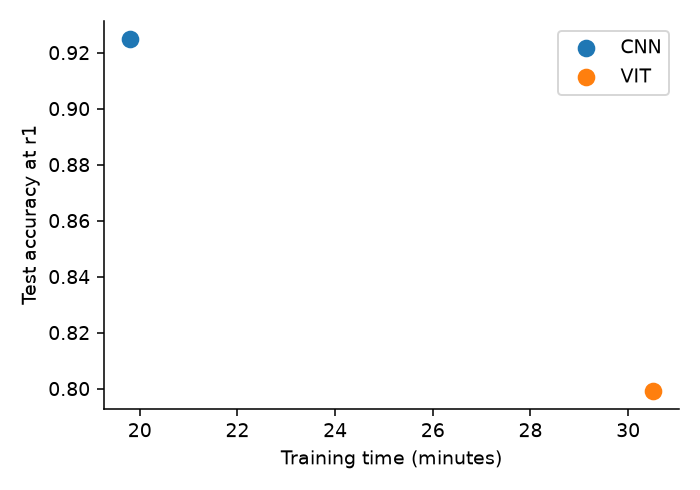
\includegraphics[width=\linewidth,height=.30\textheight,keepaspectratio]{figures/time.png}
\caption{Время обучения и test accuracy при полном train; два исходных запуска E1.}\label{fig:time}
\end{figure}

\section{E1. Эффективность по объёму данных}
Теоретическое ожидание --- преимущество локальности CNN при малом числе примеров и возможное сокращение разрыва при росте train. Для каждой доли обе модели выполняют ровно 10 000 обновлений, поэтому число проходов по малой выборке больше:
\begin{equation}E_r\approx S/\lceil n_r/B\rceil.\end{equation}
$n_r$ --- число обучающих изображений, $B=128$. В таблице показано фактически обработанное число эквивалентных эпох; различия последнего неполного batch учитываются журналом.
\begin{table}[H]\centering\small
\setlength{\tabcolsep}{4pt}
\caption{E1: validation и test при общем бюджете 10 000 обновлений.}\label{tab:e1}
\begin{tabular}{lrrrrrl}
\toprule
Модель & $r$ & $n_r$ & Val acc. & Test acc. & $E_r$ & Источник \\
\midrule
CNN & 0.05 & 2150 & 0.7130 & 0.7074 & 588.24 & R01 \\
VIT & 0.05 & 2150 & 0.4562 & 0.4502 & 588.24 & R02 \\
CNN & 0.15 & 6450 & 0.8462 & 0.8378 & 196.08 & R03 \\
VIT & 0.15 & 6450 & 0.5952 & 0.5914 & 196.08 & R04 \\
CNN & 0.3 & 12900 & 0.8884 & 0.8799 & 99.01 & R05 \\
VIT & 0.3 & 12900 & 0.6886 & 0.6879 & 99.01 & R06 \\
CNN & 0.6 & 25800 & 0.9150 & 0.9070 & 49.51 & R07 \\
VIT & 0.6 & 25800 & 0.7740 & 0.7601 & 49.51 & R08 \\
CNN & 1.0 & 43000 & 0.9324 & 0.9250 & 29.76 & R09 \\
VIT & 1.0 & 43000 & 0.8030 & 0.7991 & 29.76 & R10 \\
\bottomrule
\end{tabular}
\end{table}


\begin{figure}[H]\centering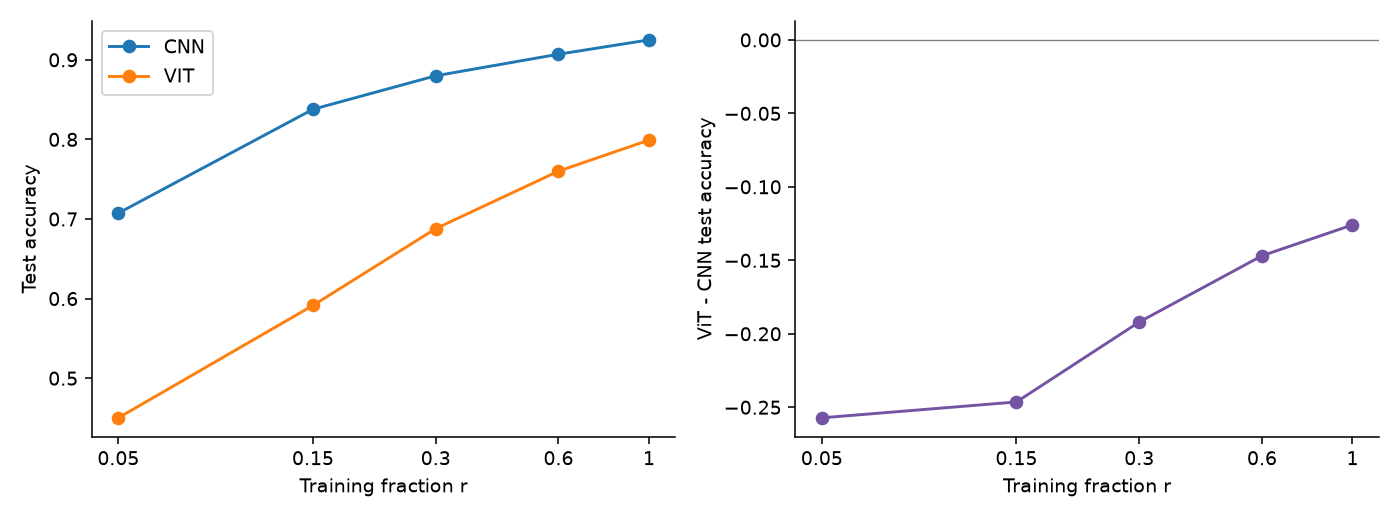
\includegraphics[width=\linewidth,height=.38\textheight,keepaspectratio]{figures/learning.png}
\caption{Test accuracy и разность ViT минус CNN в зависимости от доли данных; источники приведены в таблице E1.}\label{fig:learning}
\end{figure}

Разность ViT минус CNN изменилась от $-0.2572$ при $r=0.05$ до $-0.1259$ при $r=1$. Разрыв сократился на 0.1313, но лидер не сменился ни на одной доле; $r^*$ в измеренном диапазоне отсутствует. Нельзя продолжать кривую за $r=1$ без новых данных. Увеличение данных здесь одновременно уменьшает число повторных проходов при фиксированном $S$.
\begin{figure}[H]\centering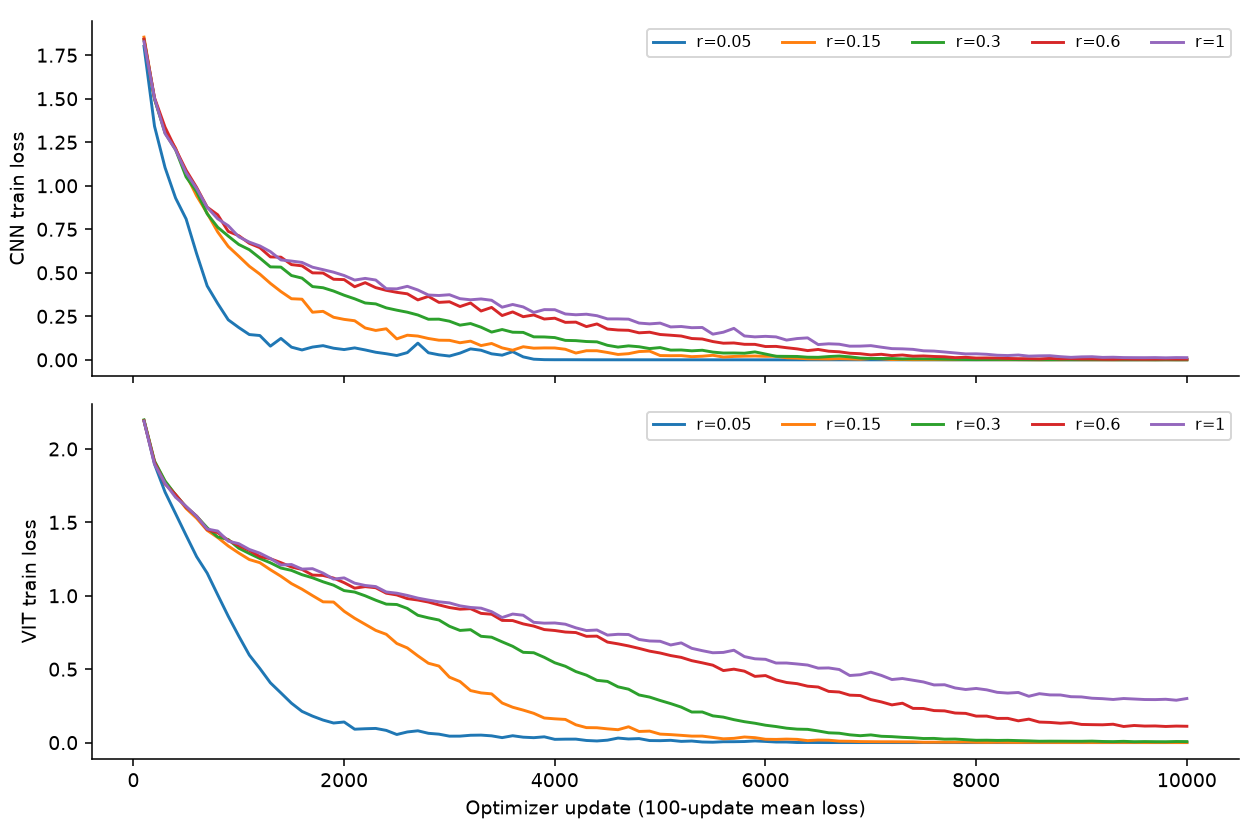
\includegraphics[width=\linewidth,height=.47\textheight,keepaspectratio]{figures/loss.png}
\caption{Сохранённые train loss всех условий E1 при одинаковом числе обновлений.}\label{fig:loss}
\end{figure}

\section{E2. Искажения тестовых изображений}
Использованы фиксированные полные модели E1, CNN R09 и ViT R10. Все преобразования выполнены в RGB $[0,1]$ до нормализации, затем значения ограничены этим диапазоном. Blur: $\sigma=0.5,1,1.5$ и ядра 5,7,11; contrast: коэффициенты 0.6,0.4,0.2 относительно средней яркости; patch shuffle: стороны блока 16,8,4. При $s=0$ вход тождествен чистому. Обе архитектуры получают одни и те же случайные преобразования каждого test-изображения.
\begin{table}[H]\centering\small
\setlength{\tabcolsep}{4pt}
\caption{E2: точность и относительное падение качества на test; веса полных моделей фиксированы.}\label{tab:e2}
\begin{tabular}{lrrrrr}
\toprule
Искажение & $s$ & $M_{CNN}$ & $M_{ViT}$ & $\delta_{CNN}$ & $\delta_{ViT}$ \\
\midrule
blur & 0 & 0.9250 & 0.7991 & 0.0000 & 0.0000 \\
blur & 1 & 0.9163 & 0.7685 & 0.0094 & 0.0383 \\
blur & 2 & 0.3544 & 0.4972 & 0.6169 & 0.3778 \\
blur & 3 & 0.2012 & 0.3534 & 0.7825 & 0.5578 \\
contrast & 0 & 0.9250 & 0.7991 & 0.0000 & 0.0000 \\
contrast & 1 & 0.9101 & 0.6992 & 0.0161 & 0.1250 \\
contrast & 2 & 0.8570 & 0.4685 & 0.0735 & 0.4137 \\
contrast & 3 & 0.5476 & 0.2028 & 0.4080 & 0.7462 \\
patch shuffle & 0 & 0.9250 & 0.7991 & 0.0000 & 0.0000 \\
patch shuffle & 1 & 0.6346 & 0.5739 & 0.3139 & 0.2818 \\
patch shuffle & 2 & 0.3462 & 0.5700 & 0.6257 & 0.2867 \\
patch shuffle & 3 & 0.2055 & 0.5705 & 0.7778 & 0.2861 \\
\bottomrule
\end{tabular}
\end{table}


\begin{table}[H]\centering\small
\setlength{\tabcolsep}{4pt}
\caption{Среднее качество по трём ненулевым уровням и смена лидера.}\label{tab:means}
\begin{tabular}{lrrrl}
\toprule
Искажение & $\overline M_{CNN}$ & $\overline M_{ViT}$ & $\Delta$ & Смена \\
\midrule
blur & 0.490633 & 0.539700 & +0.049067 & да \\
contrast & 0.771567 & 0.456833 & -0.314733 & нет \\
patch shuffle & 0.395433 & 0.571467 & +0.176033 & да \\
\bottomrule
\end{tabular}
\end{table}


\begin{figure}[H]\centering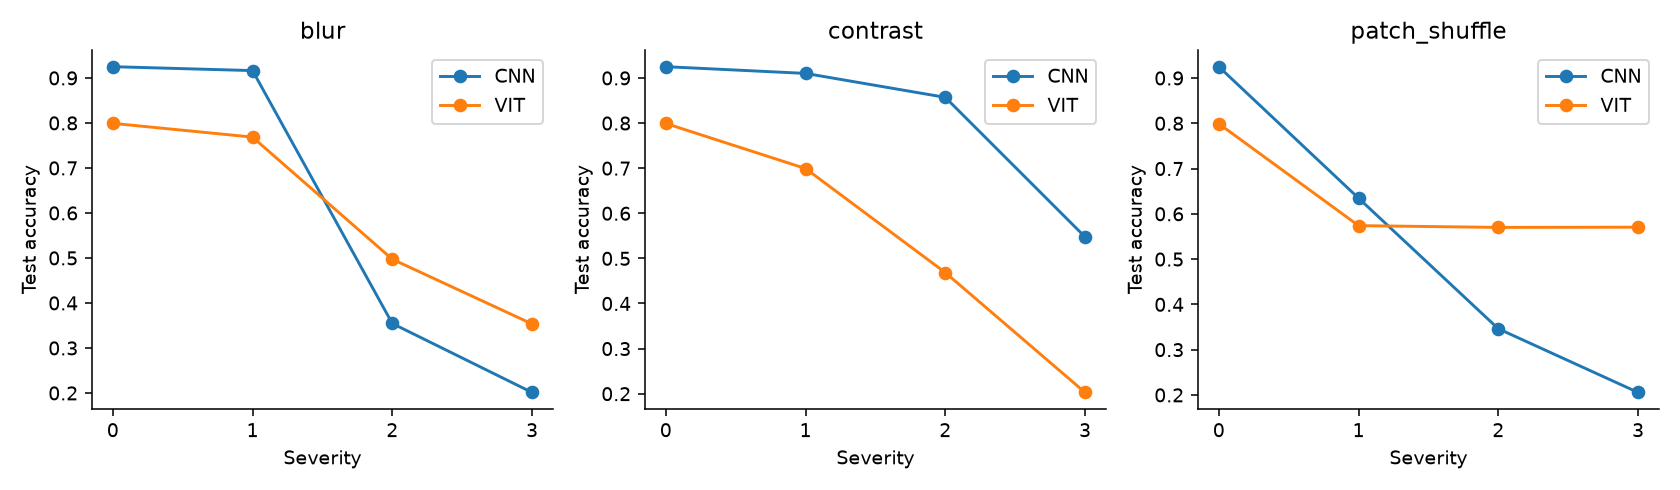
\includegraphics[width=\linewidth,height=.39\textheight,keepaspectratio]{figures/corruptions.png}
\caption{Изменение точности при трёх искажениях персонального профиля; веса не переобучаются.}\label{fig:corruptions}
\end{figure}

На чистом test преимущество CNN равно 0.1259. Для blur средняя разность ViT минус CNN положительна, 0.049067, для patch shuffle --- 0.176033: в обоих случаях выполнено правило смены лидера. Contrast сохраняет преимущество CNN, средняя разность $-0.314733$. Это показывает зависимость качества от типа сдвига. Перестановка блоков разрушает локальную структуру CNN; для ViT она меняет позиции токенов, но не содержимое патча $4\times4$. Обучаемые абсолютные позиции не позволяют объявить ViT строго инвариантным к перестановке.

\section{E3 и карта относительного преимущества}
Режим E3 выбран по максимальному модулю разности на val: $r=0.05$, исходная разность $-0.2568$. До дополнительных seed зафиксирована гипотеза о сохранении отрицательного знака и близкой величины на test. Одинаковы подмножество, A1, $S$, batch, архитектуры и выбранные LR; меняются только общие seed 1,2,3. Seed 1 соответствует E1 и явно повторно используется.
\begin{table}[H]\centering\small
\setlength{\tabcolsep}{4pt}
\caption{E3: все парные результаты на доле $r=0.05$.}\label{tab:e3}
\begin{tabular}{lrrrl}
\toprule
Seed & CNN & ViT & $\Delta_s$ & Источники \\
\midrule
1 & 0.7074 & 0.4502 & -0.257200 & R01/R02 \\
2 & 0.6884 & 0.4587 & -0.229700 & R11/R12 \\
3 & 0.7123 & 0.4508 & -0.261500 & R13/R14 \\
\bottomrule
\end{tabular}
\end{table}


Для $\Delta_s=M_{ViT,s}-M_{CNN,s}$ среднее равно $-0.249467$, выборочное SD --- 0.017253. Все три разности отрицательны, а $|\overline\Delta|>2s_\Delta=0.034506$: различие установлено в пользу CNN. Отклонение среднего от численной гипотезы $-0.2568$ составляет +0.007333. Направление ожидания подтверждено.
\begin{figure}[H]\centering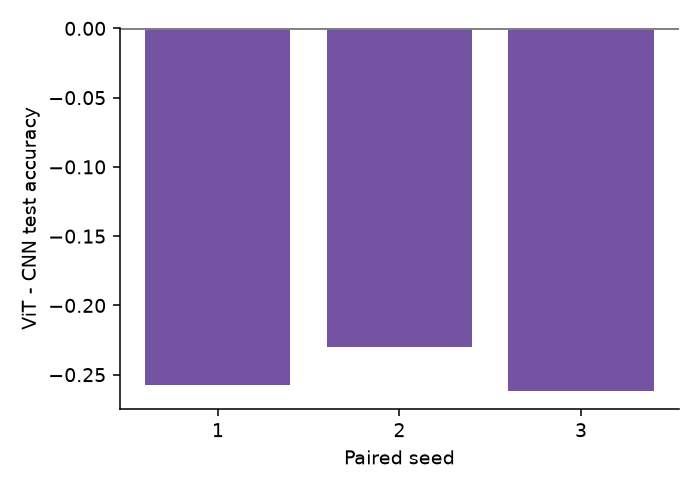
\includegraphics[width=\linewidth,height=.28\textheight,keepaspectratio]{figures/paired.png}
\caption{Все три парные разности E3. Положительное значение означало бы преимущество ViT.}\label{fig:paired}
\end{figure}

\begin{figure}[H]\centering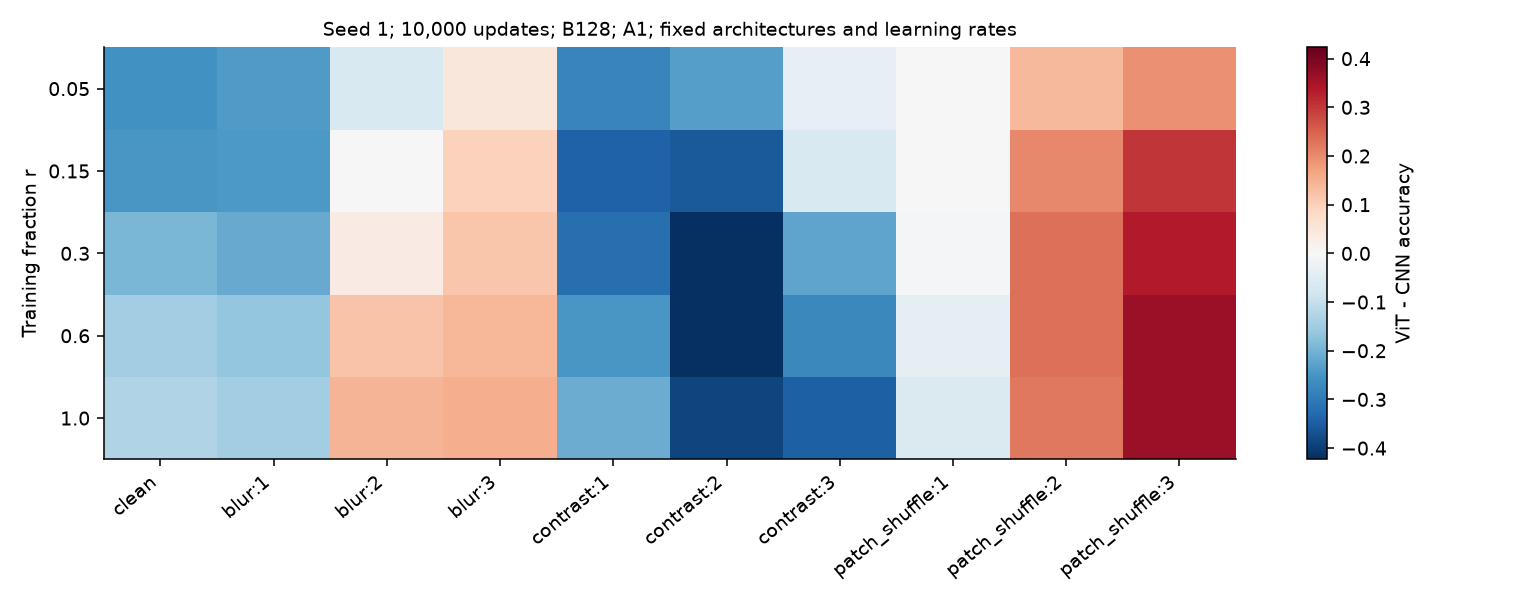
\includegraphics[width=\linewidth,height=.47\textheight,keepaspectratio]{figures/map.png}
\caption{Карта относительного преимущества: доля train и условие test; фиксированы модели, A1, бюджет и seed 1.}\label{fig:map}
\end{figure}

В карте меняются доля train и условие test; фиксированы A1, бюджет, рецепты оптимизации и seed 1. Это двумерный срез, а не сравнение после подбора по test. Три seed E3 описывают вариативность обучения на одном подмножестве; смену split и рецепта они не охватывают.

\section{Ответы на контрфактические вопросы и выводы}
\subsection*{Вопрос 1. Рост объёма данных}
Разность изменилась с $-0.2572$ до $-0.1259$ (R01/R02 и R09/R10), то есть на +0.1313. Это сокращение разрыва не предсказывает знак при большем датасете: train CIFAR-10 исчерпан. Локальность, общие веса, A1, конечный бюджет и выбранные LR могут сохранять преимущество CNN; эксперимент не выделяет один из этих механизмов отдельно.
\subsection*{Вопрос 2. Одинаковое число эпох вместо одинаковых шагов}
На полном train $E=10\,000/336=29.7619$. Для 2150 изображений это даёт $\lceil29.7619\cdot17\rceil=506$ шагов. Сохранённый дополнительный опыт CNN дал test accuracy 0.6169 против 0.7074 при 10 000 шагах: падение 0.0905. Меняется и число предъявлений, и горизонт cosine с прогревом, поэтому это не чистая оценка одного механизма. Источник: R15.
\subsection*{Вопрос 3. Параметры и вычислительный бюджет}
По исходным профилям отношение параметров ViT/CNN равно 0.957186, MAC --- 1.279649, времени обучения --- 1.540765. Режим равных параметров выполнен, равных вычислений --- нет. Число параметров не определяет цену внимания и пропускную способность.
\subsection*{Вопрос 4. Уменьшение патча вдвое}
Для $P=4$ имеется $N'=65$, для $P=2$ --- 257 токенов. Стоимость блока выросла с 118 260 480 до 505 479 936 MAC; квадратичный член --- в $(257/65)^2=15.632899$ раза. Полная модель с $P=2$ имеет 10 755 466 параметров, лишь в 1.005601 раза больше исходной. Размеры весов блоков зависят от $D$, а не числа токенов; меняются patch projection и таблица позиций. Значения подтверждены сохранённым профилированием R16, обучения этой модификации не заявляется.
\subsection*{Вопрос 5. Сдвиги на 2, 4 и 8 пикселей}
\begin{table}[H]\centering\small
\setlength{\tabcolsep}{4pt}
\caption{Дополнительная оценка сдвигов без переобучения полных моделей.}\label{tab:translation}
\begin{tabular}{rrrrr}
\toprule
Сдвиг, пикс. & CNN accuracy & ViT accuracy & Падение CNN & Падение ViT \\
\midrule
2 & 0.9270 & 0.7987 & -0.0020 & +0.0004 \\
4 & 0.9194 & 0.7887 & +0.0056 & +0.0104 \\
8 & 0.8924 & 0.7271 & +0.0326 & +0.0720 \\
\bottomrule
\end{tabular}
\end{table}


Сдвиги 4 и 8 кратны патчу ViT, только 8 кратен общему stride CNN. Однако 8 пикселей дают наибольшее среднее падение, 0.0523, против $-0.0008$ и 0.0080 при 2 и 4. A1 покрывает сдвиги 2/4, но не 8; границы изображения, padding и pooling также нарушают строгую инвариантность классификации. Поэтому простая кратность stride не объясняет результат, а вклад аугментации нельзя отделить от величины сдвига по этим трём точкам.
\noindent\textbf{Заключение.} CNN точнее ViT на всех долях train, а при 5\% данных это подтверждено на трёх seed. Blur и patch shuffle меняют лидера. Преимущество зависит от условий; равенство параметров не означает равенства вычислений.
\clearpage
\renewcommand{\refname}{Список использованных источников}
\begin{thebibliography}{9}
\addcontentsline{toc}{section}{Список использованных источников}
\bibitem{teacher} Лабораторная работа 2. Архитектурные inductive biases в компьютерном зрении. CNN vs Vision Transformer: sample efficiency, augmentation, transfer и distribution shift. Курс «Нейронные сети». Методические указания, 2026.
\end{thebibliography}
\clearpage
\section*{Приложение. Идентификация запусков}
\addcontentsline{toc}{section}{Приложение. Идентификация запусков}
\begingroup\small\setstretch{1.05}
\begin{longtable}{@{}l>{\raggedright\arraybackslash}p{3.5cm}p{10.8cm}@{}}
\caption{Полные RUN\_ID источников результатов.}\\
\toprule Код & Условие & RUN\_ID \\ \midrule \endhead
\hypertarget{R01}{R01} & CNN r0.05 s1 & {\fontsize{8.8}{11}\selectfont\texttt{8705d516f9c58ae4458c-2297f86c299c4b998e5a33258a6b8326}} \\
\hypertarget{R02}{R02} & VIT r0.05 s1 & {\fontsize{8.8}{11}\selectfont\texttt{76a6bee7ce9731bfa4fa-8edbe989a96e427c82f75e87ddd2c0ab}} \\
\hypertarget{R03}{R03} & CNN r0.15 s1 & {\fontsize{8.8}{11}\selectfont\texttt{b50b6ea8552d63768374-4d1f73742ac24869a8d8cee0b7cfcc77}} \\
\hypertarget{R04}{R04} & VIT r0.15 s1 & {\fontsize{8.8}{11}\selectfont\texttt{495f34d7f6c639e46a93-9104dc9ff56f47f5aab182fd287ed1a8}} \\
\hypertarget{R05}{R05} & CNN r0.3 s1 & {\fontsize{8.8}{11}\selectfont\texttt{5b5befc1e4def983b9ee-22c1988662a44a8c9b33328924f411ab}} \\
\hypertarget{R06}{R06} & VIT r0.3 s1 & {\fontsize{8.8}{11}\selectfont\texttt{29176cb8f39f6f4d8171-6885d00915674ed3ade5cd94f2531767}} \\
\hypertarget{R07}{R07} & CNN r0.6 s1 & {\fontsize{8.8}{11}\selectfont\texttt{1127217ff6ad88909e85-a8b568720c0c4b4ea2f2098459e6ec33}} \\
\hypertarget{R08}{R08} & VIT r0.6 s1 & {\fontsize{8.8}{11}\selectfont\texttt{f154afa0aa4ee77b3250-ea30b6ab3cf942eab4e96026e089f583}} \\
\hypertarget{R09}{R09} & CNN r1.0 s1 & {\fontsize{8.8}{11}\selectfont\texttt{cfd869bd9ae49d9e218c-674bd37aac074d9393378ce924e7c6dc}} \\
\hypertarget{R10}{R10} & VIT r1.0 s1 & {\fontsize{8.8}{11}\selectfont\texttt{766dbdc705ebc387709a-0ecabc3039f24a5f872dd82e7d55734b}} \\
\hypertarget{R11}{R11} & CNN r0.05 s2 & {\fontsize{8.8}{11}\selectfont\texttt{f1a84ec3e8723294d4a2-14cad9141a774b6daee3100c969640f6}} \\
\hypertarget{R12}{R12} & VIT r0.05 s2 & {\fontsize{8.8}{11}\selectfont\texttt{1620cd8ad55b41c9e6c2-7e9c1d9d13e44a5bbee06a6bc7693cac}} \\
\hypertarget{R13}{R13} & CNN r0.05 s3 & {\fontsize{8.8}{11}\selectfont\texttt{69ac6bd9ed94ae61d1aa-873bbd5089054e138a586cd2a337e139}} \\
\hypertarget{R14}{R14} & VIT r0.05 s3 & {\fontsize{8.8}{11}\selectfont\texttt{793fe73a531b8002205c-4bc06191663d459e941756cc0e6a26b1}} \\
\hypertarget{R15}{R15} & CF2 CNN 506 steps & {\fontsize{8.8}{11}\selectfont\texttt{d1a718622a886ab7d1fd-42792e1b10654612a8812f0182aee6f1}} \\
\hypertarget{R16}{R16} & CF4 P2 profiling & {\fontsize{8.8}{11}\selectfont\texttt{3f22804f8649bd648df6-65596ace07164264a7d02cf72f8804d1}} \\
\bottomrule\end{longtable}\endgroup
